% Created 2020-08-16 Sun 13:15
% Intended LaTeX compiler: pdflatex
\documentclass[presentation]{beamer}
\usepackage[utf8]{inputenc}
\usepackage[T1]{fontenc}
\usepackage{graphicx}
\usepackage{grffile}
\usepackage{longtable}
\usepackage{wrapfig}
\usepackage{rotating}
\usepackage[normalem]{ulem}
\usepackage{amsmath}
\usepackage{textcomp}
\usepackage{amssymb}
\usepackage{capt-of}
\usepackage{hyperref}
\usetheme{UoB}
\author{Mark Blyth}
\date{}
\title{Paper + some CBC results}
\hypersetup{
 pdfauthor={Mark Blyth},
 pdftitle={Paper + some CBC results},
 pdfkeywords={},
 pdfsubject={},
 pdfcreator={Emacs 26.3 (Org mode 9.1.9)}, 
 pdflang={English}}
\begin{document}

\maketitle

\section{Background}
\label{sec:org69f5c53}
\begin{frame}[label={sec:org2244324}]{Week's goal}
\begin{itemize}
\item Play with in-silico CBC
\item Write conference paper
\end{itemize}
\end{frame}
\section{CBC}
\label{sec:orgd99d698}
\begin{frame}[label={sec:org7f8ef3b}]{Fourier, Duffing}
\begin{center}
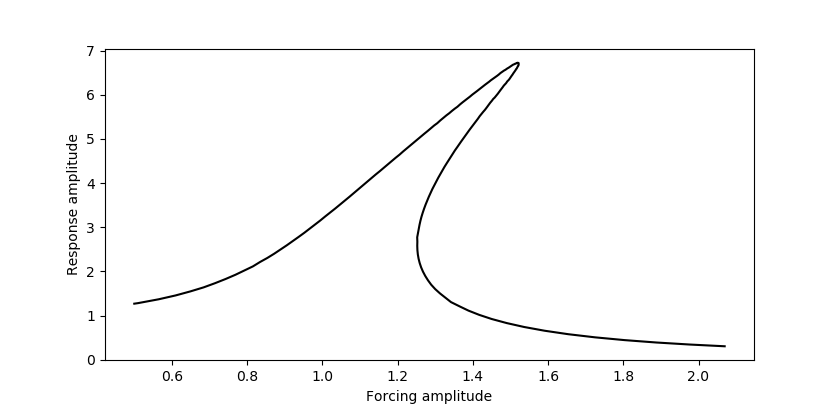
\includegraphics[width=.9\linewidth]{./success.png}
\end{center}
\end{frame}

\begin{frame}[plain,label={sec:org860df28}]{XPP Fitzhugh-Nagumo}
\begin{center}
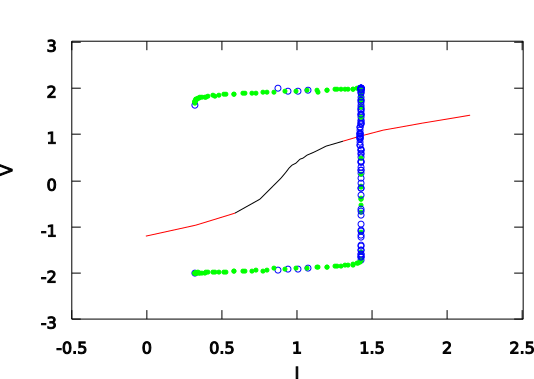
\includegraphics[width=.9\linewidth]{./fh_bifurcation.png}
\end{center}
\end{frame}

\begin{frame}[label={sec:orga12818d}]{Modified Fitzhugh-Nagumo model}
\begin{columns}
\begin{column}{0.5\columnwidth}
\begin{block}{Original}
\begin{align}
\dot{v} &= v - v^3/3 - w + I\\
\dot{w} &= 0.08(v + 0.7 - 0.8w)
\end{align}
\end{block}
\end{column}

\begin{column}{0.5\columnwidth}
\begin{block}{New}
\begin{align}
\dot{v} &= v - v^3/3 - w + I\\
\dot{w} &= 0.8(v + 0.7 - 0.8w)
\end{align}
\end{block}
\end{column}
\end{columns}

\vfill

\begin{itemize}
\item Changed timescale separation
\item `Widens out' Canard explosion
\item Makes signal less nonlinear, more readily described with Fourier
\end{itemize}
\end{frame}

\begin{frame}[plain,label={sec:org2900f7b}]{XPP modified}
\begin{center}
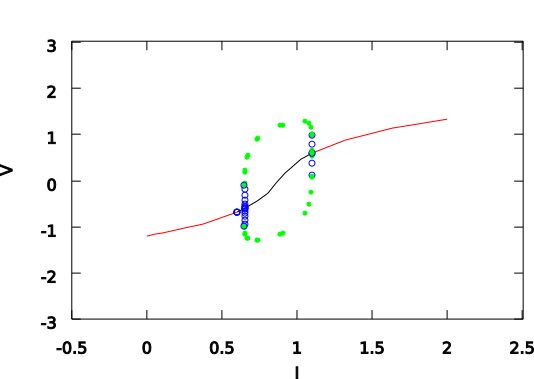
\includegraphics[width=.9\linewidth]{./modified_FH_bifurcation.png}
\end{center}
\end{frame}

\begin{frame}[label={sec:org4c3586e}]{Modified Fitzhugh-Nagumo CBC}
\begin{center}
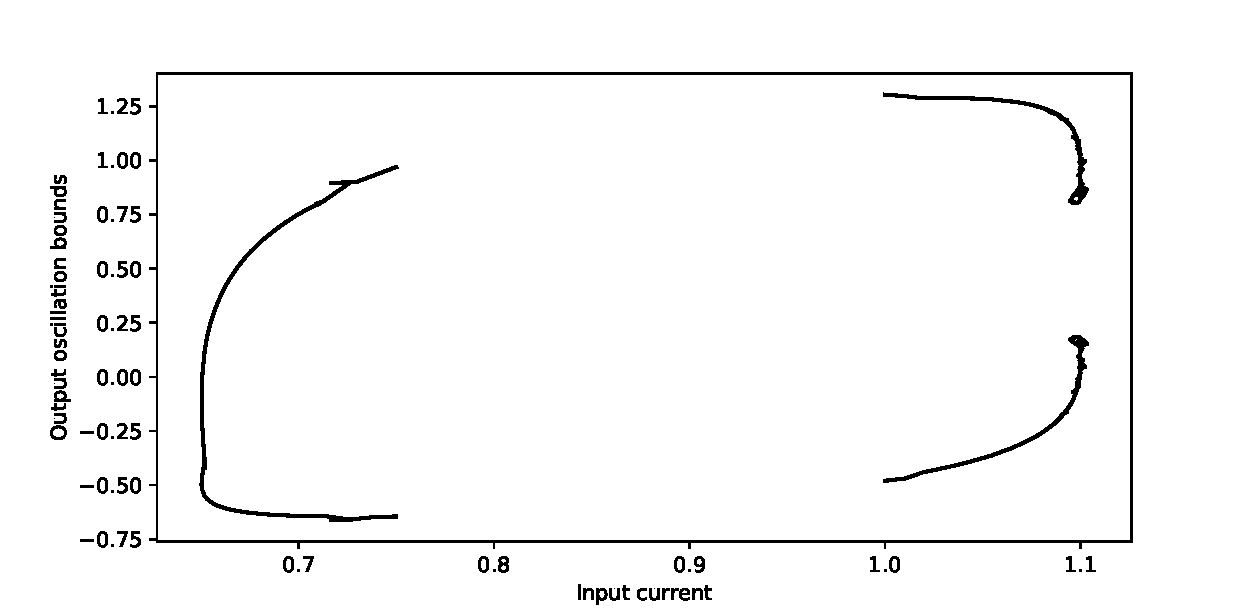
\includegraphics[width=.9\linewidth]{./simplified_FH_CBC_2.pdf}
\end{center}
\end{frame}


\begin{frame}[label={sec:org56234e0}]{Modified Fitzhugh-Nagumo CBC}
\begin{center}
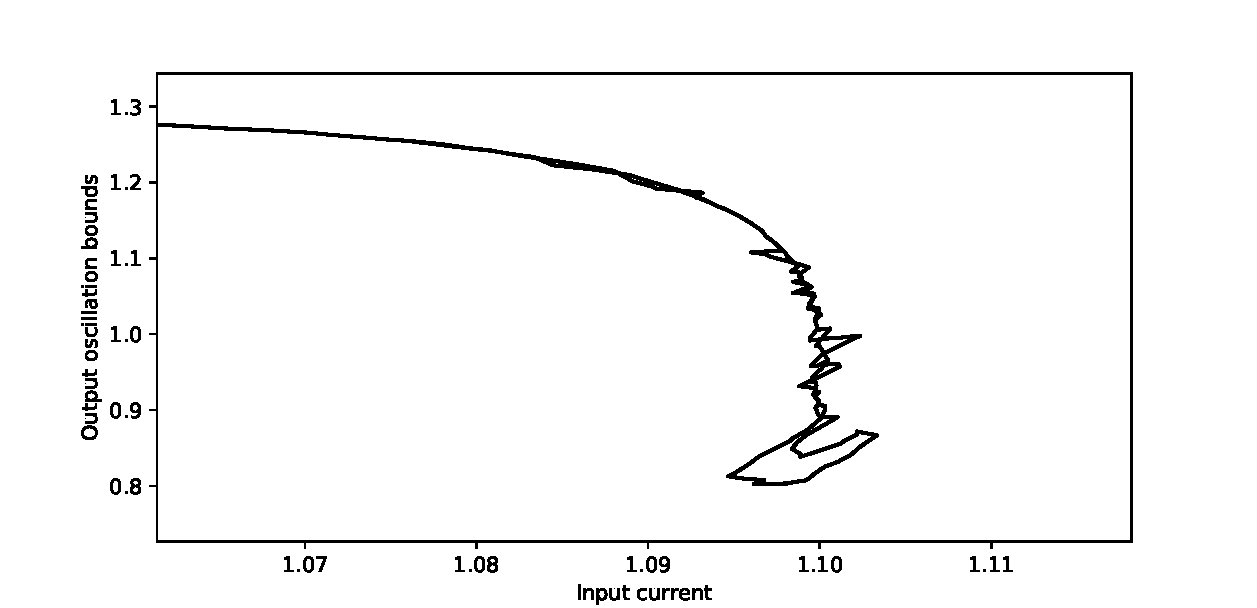
\includegraphics[width=.9\linewidth]{./simplified_FH_CBC_zoom.pdf}
\end{center}
\end{frame}

\begin{frame}[<+->][label={sec:orgc58b339}]{CBC progress}
DONE:
\begin{itemize}
\item IO-map method for (harmonically forced) Duffing, Fourier discretisation
\begin{itemize}
\item No phase constraint; signal period taken from forcing parameter
\end{itemize}
\item IO-map method for modified Fitzhugh-Nagumo model, Fourier discretisation
\begin{itemize}
\item Phase constraint; signal period treated as continuation parameter
\end{itemize}
\end{itemize}

\vfill
TODOs:
\begin{itemize}
\item CBC with splines discretisation
\item CBC using the `other' (non-IO-map) method
\item CBC on the equilibrium
\end{itemize}
\end{frame}

\section{Paper}
\label{sec:org985d764}
\begin{frame}[plain,label={sec:orgd66ee85}]{Conference paper}
Currently drafted:
\begin{itemize}
\item Intro
\item Maths behind CBC, plus motivation of discretisation
\item Novel discretisation methods
\end{itemize}
\vfill
TODOs:
\begin{itemize}
\item Surrogate models as adaptive filters for cleaner Fourier discretisation
\item Usage cases of surrogates, novel discretisors
\begin{itemize}
\item Might merge with conclusion or intro
\end{itemize}
\item Conclusion
\item Figures
\item Proof-reading / editing / re-drafting
\end{itemize}
\end{frame}
\section{Next steps}
\label{sec:org8d6d70b}
\begin{frame}[label={sec:org7b5bc31}]{Next steps}
\begin{enumerate}
\item Write paper
\begin{itemize}
\item Goal: finish text by Friday
\end{itemize}
\item Generate figs for paper
\begin{itemize}
\item Splines vs. Fourier: goodness-of-fit vs. dimensionality of discretisation
\item Splines vs. Fourier: noise-robustness
\item Plus any figs for the surrogates section
\end{itemize}
\item Proof read, re-draft, edit paper
\item Implement a splines-based CBC
\begin{itemize}
\item Not essential, but paper would benefit from saying we've done it
\item Best to get a completed paper first, then start on this
\end{itemize}
\end{enumerate}
\end{frame}
\end{document}
